\PassOptionsToPackage{table}{xcolor}
\documentclass[lettersize,journal]{IEEEtran}
\usepackage[caption=false,font=footnotesize]{subfig}
  
\usepackage{ragged2e}
\usepackage{caption}
\captionsetup{justification=centering}

\usepackage{algorithm}
\usepackage{algpseudocode}
\usepackage{array}
% \usepackage[caption=false,font=normalsize,labelfont=sf,textfont=sf]{subfig}
\usepackage{textcomp}
\usepackage{stfloats}
\usepackage{url}
\usepackage{verbatim}
\usepackage{graphicx}
\usepackage{cite}
\usepackage[utf8]{inputenc}
\usepackage{tikz}
\usepackage{float}
\usepackage{forest}
\usetikzlibrary{arrows.meta, shapes.geometric, positioning, fit, backgrounds}
\usepackage{booktabs}
\usepackage{multirow}
\usepackage{amsmath,amssymb,amsfonts}\usepackage{dsfont}
% Algorithms
%\usepackage[linesnumbered,ruled,vlined]{algorithm2e}
% \usepackage{algorithmicx}
\usepackage{academicons} % for ORCID icon
\usepackage[table]{xcolor}     % to color the icon
\definecolor{limegreen}{RGB}{50,205,50}
\newcommand{\orcid}[1]{\href{https://orcid.org/#1}{\textcolor{limegreen}{\aiOrcid}}}
\usepackage{hyperref}
\usepackage{algpseudocode}
\usepackage{tabularx}
\usepackage{caption}
\usepackage{bm}
% \usepackage[caption=false,font=normalsize,labelfont=sf,textfont=sf]{subfig}
\newcommand{\mask}{\texttt{[MASK]}}

\hyphenation{op-tical net-works semi-conduc-tor IEEE-Xplore}
% updated with editorial comments 8/9/2021

\begin{document}

\title{Diffusion-based Large Language Models Survey}

\author{Chiung-Yi Tseng, Danyang Zhang, Junhao Song, Ziqian Bi% <-this % stops a space
\thanks{Chiung-Yi Tseng and Danyang Zhang are with the AI Agent Lab, Vokram Group, London, United Kingdom (e-mails: ctseng@luxmuse.ai, danyang@vokram.com). Junhao Song is with the Department of Computing, Imperial College London, London, United Kingdom (email: junhao.song23@imperial.ac.uk). Ziqian Bi is with the Department of Computer Science, Purdue University, West Lafayette, Indiana, United States (email: bi32@purdue.edu).}% <-this % stops a space
\thanks{Corresponding author: Junhao Song (junhao.song23@imperial.ac.uk)}
}

% \IEEEpubid{0000--0000/00\$00.00~\copyright~2021 IEEE}
% Remember, if you use this you must call \IEEEpubidadjcol in the second
% column for its text to clear the IEEEpubid mark.

\maketitle

\begin{abstract}
Diffusion-based large language models (DLLMs) have emerged as a promising alternative to traditional autoregressive architectures, notably enhancing parallel generation, controllability, and robustness across multiple modalities. Originally developed from continuous diffusion methods in computer vision, recent adaptations of DLLMs have tailored discrete diffusion processes through absorbing-state kernels, latent projections, and hybrid architectures. This survey reviews recent developments in DLLMs, beginning with their foundational concepts, including DDPM, DDIM, and their early discrete adaptations, such as mask-based, continuous-embedding, and hybrid models. We organize current methods by sampling strategy, guidance type, noise schedule, and temporal conditioning, and analyzes their efficiency, output quality, and fine-tuning. The paper also highlights key advancements: autoregressive-diffusion unification through hyperschedules, adaptive correction sampling, and efficient caching mechanisms to enhance computational performance. Besides, it explores emerging applications, such as natural language tasks, multimodal generation, and reasoning-intensive domains... These demonstrate the versatility of DLLMs. Furthermore, the paper identifies critical challenges, including adaptive sampling, scalable alignment strategies, deeper integration with pretrained language models, graph-based diffusion frameworks, and robust evaluation protocols. Finally, the paper proposes directions that could define future research in diffusion-based sequence generation.
\end{abstract}

\begin{IEEEkeywords}
Diffusion large language models, discrete denoising, large language models, latent diffusion, multimodal generation
\end{IEEEkeywords}

\section{Evolution of Diffusion Language Models}
\label{sec:evolution}
\IEEEPARstart{D}{iffusion}-based language models (DLLMs) have rapidly advanced from their thermodynamic origins to versatile generators across modalities. We trace this evolution in four stages.

\begin{figure}[ht!]
    \centering
    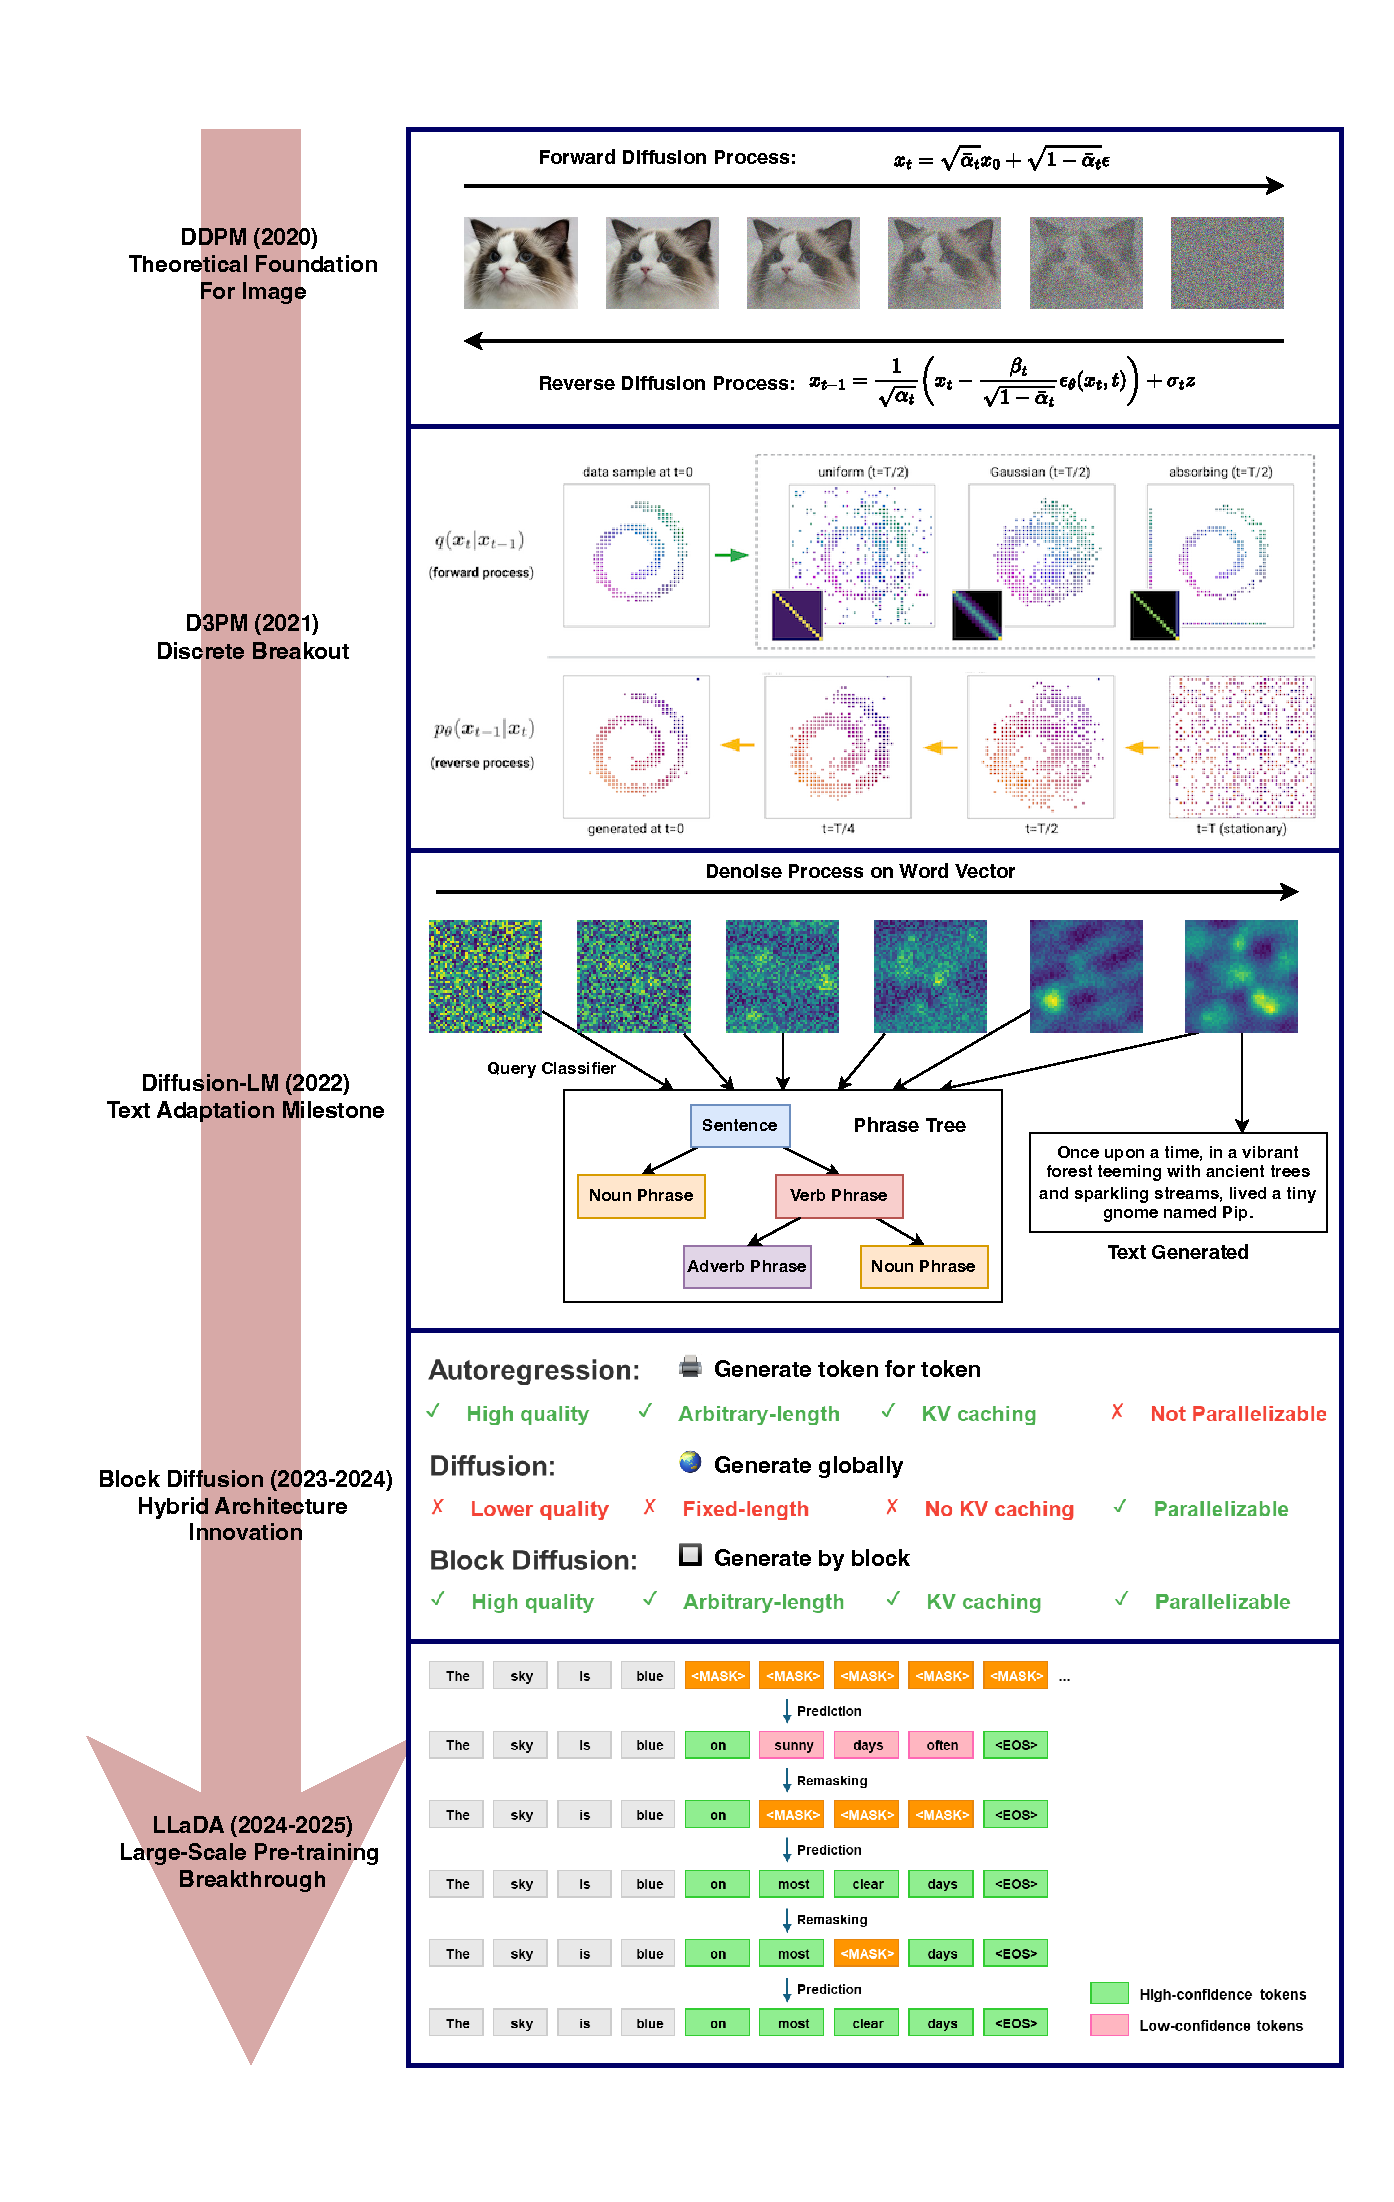
\includegraphics[width=0.95\linewidth]{figs/diffusion.pdf}
    \caption{\centering Evolution timeline of major diffusion model breakthroughs (2020-2025), demonstrating the progression from foundational frameworks to advanced hybrid architectures in generative model.}
    \label{fig:diffusion}
\end{figure}

\begin{figure*}[t]
    \centering
    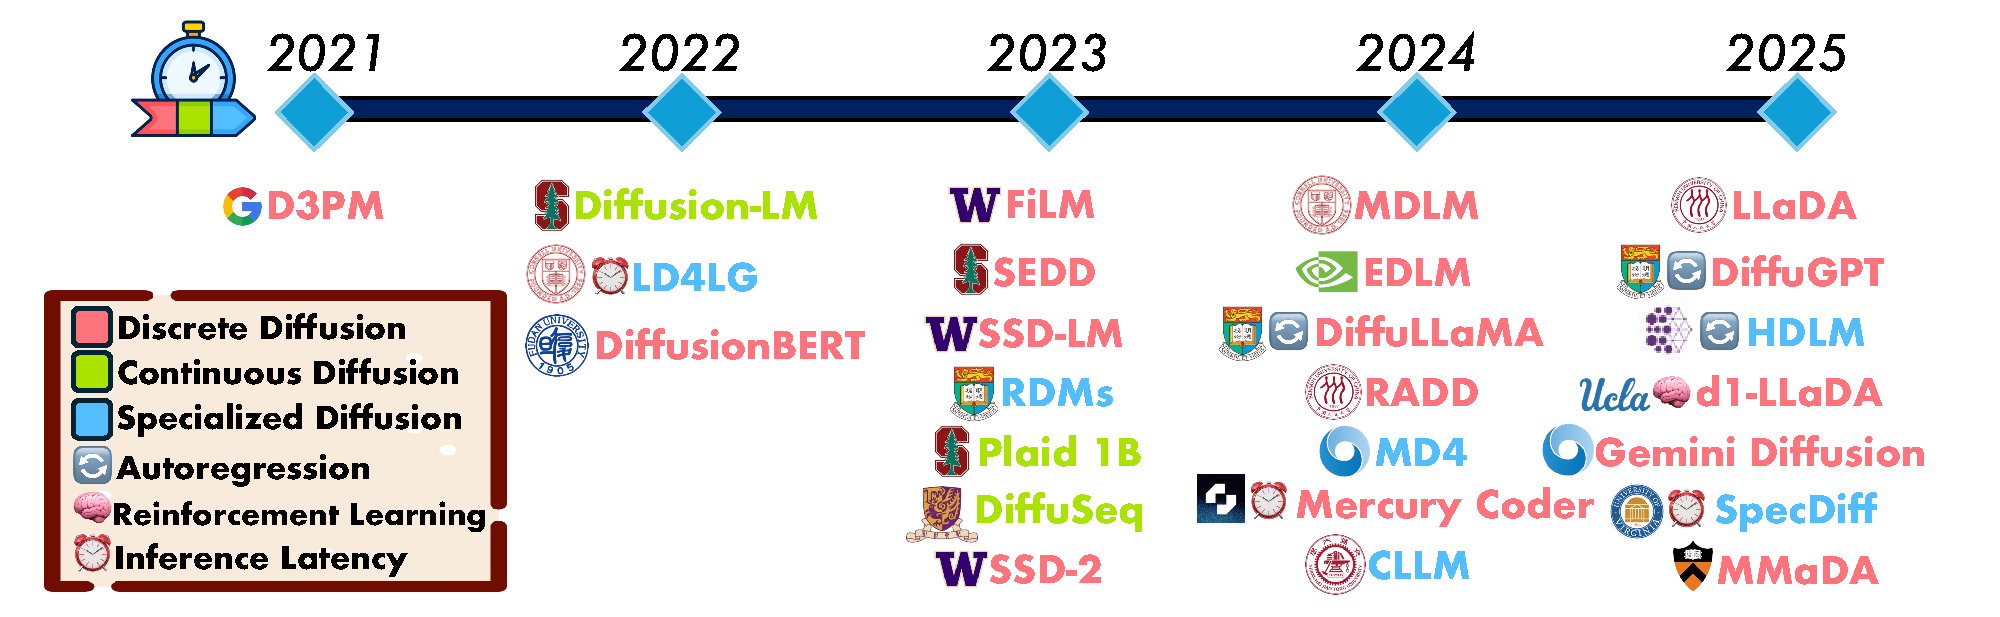
\includegraphics[width=0.95\textwidth]{figs/DLLMs_timeline.pdf}
    \caption{Evolution of key Diffusion Language Models (DLLMs) from 2021 to 2025, annotated by architectural innovations (e.g., discrete/continuous diffusion), integration with autoregression or reinforcement learning, and inference efficiency breakthroughs.}
    \label{fig:timeline}
\end{figure*}

\subsection{Early Foundations (2015–2020)}
The original \textbf{Denoising Diffusion Probabilistic Models (DDPM)} introduced a Markovian forward and reverse noising chain on continuous data, establishing the core variational framework for diffusion-based generation \cite{ho_denoising_2020}. Building on this, \textbf{Denoising Diffusion Implicit Models (DDIM)} generalized DDPM sampling to a non-Markovian family of deterministic or accelerated trajectories, while preserving the same training objective \cite{song_denoising_2020}. To handle discrete data, Hoogeboom \emph{et al.} proposed \textbf{Structured Denoising Diffusion Models in Discrete State-Spaces (D3PM)}, which uses absorbing-state kernels without explicit timestep embeddings \cite{hoogeboom_structured_2021}.

\subsection{First Text-Specific Adaptations (2021–2022)}
Zou \emph{et al.} provided the first systematic survey of diffusion for non-autoregressive text generation, defining both discrete (mask-based) and continuous (Gaussian embedding) formulations and demonstrating their parallelism and controllability advantages over prior NAR methods \cite{zou_survey_2023}. Hoogeboom’s D3PM work showed that absorbing-state discrete diffusion can produce coherent categorical samples without timestep inputs \cite{hoogeboom_structured_2021}. Concurrently, \textbf{Diffusion-LM} embedded Gaussian noise into token representations and outperformed earlier controllable generation models on sentiment and syntax tasks \cite{li_diffusion-lm_2022}. Subsequent innovations included Dieleman \emph{et al.}’s continuous diffusion on one-hot vectors with specialized rounding \cite{dieleman_continuous_2022}, Strudel \emph{et al.}’s self-conditioned embedding diffusion \cite{strudel_selfconditioned_2021}, and transformer-based ODE–diffusion hybrids such as Difformer \cite{gong_difformer_2022} and Composable Text Controls \cite{liu_composable_2022}. Han \emph{et al.} introduced SSD-LM, a semi-autoregressive simplex diffusion reducing denoising steps by half while preserving translation quality \cite{han_ssdlm_2022}, and Yuan \emph{et al.}’s SeqDiffuSeq demonstrated parallel seq2seq decoding in under 30 steps \cite{yuan_seqdiffuseq_2021}.

\subsection{Hybridization Architectural Innovations (2023–2024)}
The hybrid paradigm emerged with \textbf{}{Block Diffusion}, which interleaves autoregressive first-token sampling with blockwise diffusion to balance sequential fidelity and parallel speed \cite{arriola_block_2025}. \textbf{Latent Diffusion for Language Generation} projects token embeddings into a compact latent space for diffusion, then reconstructs via an AR decoder, achieving significant speedups without quality loss \cite{lovelace_latent_2023}. Energy-based approaches like \textbf{DiffPO} use a pretrained AR model as an energy function to reweight diffusion samples, reducing decoding error with fewer steps \cite{xu_energy-based_2025}. \textbf{Speculative Diffusion Decoding} treats a fast DLLM as a draft generator and an AR model as verifier, enabling near-AR quality with reduced sequential passes \cite{christopher_speculative_2025}. Task-specific optimizations, such as SSD-2’s inference-time fusion of small and large diffusion LMs, further improved throughput and privacy by splitting computation \cite{han_david_2024}.

\subsection{Recent Advances and Generalization (2024–2025)}
Recent work has extended DLLMs to multimodal and instruction-tuned scenarios. \textbf{HybridVLA} unifies vision, language, and action diffusion in a single model for embodied agent tasks \cite{liu_hybridvla_2025}. Studies on instruction fine-tuning, such as those by Zhou \emph{et al.}, demonstrate that diffusion LLMs can generalize zero-shot to unseen languages and tasks after English-only SFT \cite{nie_large_2025}. Comprehensive surveys highlight classification and benchmarking of DLLM capabilities across domains, marking the maturation of diffusion methods in NLP and beyond.

Together, these stages—from continuous DDPM through discrete D3PM, early NAR text diffusion, hybrid block and latent architectures, to multimodal and instruction-tuned generalists—chart the swift evolution of DLLMs into powerful, flexible generators.  

% \bibliographystyle{ieeetr}
% \bibliography{DLLM}


\section{Challenges in Diffusion-Based Text Models}
\label{sec:challenges}
DLLMs have great potential for parallelism and controllability but they also face several challenges when compared to autoregressive (AR) models. First, \textbf{inference latency} remains a significant hurdle: diffusion models often require dozens to hundreds of iterative denoising steps to produce coherent text. This causes much slower wall-clock inference times than the single-pass token sampling of AR decoders \cite{arriola_block_2025, zheng_reparameterized_2024}.

Another limitation is the \textbf{rigidity of sequence length}. Many early discrete diffusion schemes assume a fixed sequence length, making variable-length or open-ended text generation difficult without additional padding, masking strategies, or complex length prediction mechanisms \cite{arriola_block_2025, rutte_generalized_2025}.

In terms of modeling performance, diffusion-based approaches frequently underperform AR models on standard language-modeling benchmarks. This \textbf{weaker likelihood performance} arises from challenges in capturing sharp, multimodal discrete token distributions through gradual denoising processes \cite{arriola_block_2025, xu_energy-based_2025}.

Furthermore, diffusion methods can struggle with \textbf{global coherence}, as noise is often injected uniformly or blockwise across tokens. This limits the model’s ability to condition on long-range dependencies as effectively as full-attention AR decoders \cite{fathi_unifying_2025, arriola_block_2025}.

Integrating user preferences and control signals imposes additional costs: \textbf{alignment and controllability} techniques such as DiffPO require extra inference-time denoising or optimization steps to steer outputs toward desired attributes, further exacerbating latency issues \cite{chen_diffpo_2025}.

Mapping discrete text into a continuous diffusion framework introduces \textbf{encoding and reconstruction complexity}. Architectures like TEncDM rely on large projector networks to compress and reconstruct token embeddings, which can introduce errors and complicate training dynamics \cite{shabalin_tencdm_2025}.

Basic diffusion schemes also suffer from a lack of \textbf{self-correction}: once a token is denoised, early mistakes cannot be revisited without rerunning the entire process. \textbf{Generalized Interpolating Discrete Diffusion (GIDD)} addresses this by adding fixed-point resampling iterations, but at the cost of additional computation \cite{rutte_generalized_2025}.

Finally, hybrid architectures that combine AR and diffusion components—such as blockwise interpolation or hyperschedules—introduce significant \textbf{engineering complexity}. Coordinating two sampling paradigms, tuning noise schedules, and balancing error propagation across modules can dramatically increase implementation and inference overhead \cite{arriola_block_2025, fathi_unifying_2025}.

% \bibliographystyle{plain}
% \bibliography{DLLM}


\section{Categorization Criteria for Diffusion Language Models}
\label{sec:categorization_methods}
\begin{table*}[ht!]
  \centering
  \caption{Comprehensive Categorization of DLLMs (Sorted by Year and Type)}
  \label{tbl:dllm-comprehensive}
  \begin{tabularx}{\textwidth}{X  X  X  >{\RaggedRight\hyphenpenalty=50\tolerance=1000}X  c  c}
    \toprule
    \textbf{Model} & \textbf{Markovity} & \textbf{Guidance} & \textbf{Annealing Method} & \textbf{Time-Embedding} & \textbf{Type} \\
    \midrule

    Diffusion-LM \cite{li_diffusion-lm_2022}
      & Non-Markovian (embedding space)
      & Classifier-Free
      & Gaussian schedule over continuous token embeddings
      & Yes
      & Continuous \\

    Difformer \cite{gong_difformer_2022}
      & Non-Markovian (ODE sampling)
      & Classifier-Free
      & Continuous-time ODE trajectories
      & Yes
      & Continuous \\

    Composable Text Controls \cite{liu_composable_2022}
      & Non-Markovian (latent ODE)
      & Classifier-Free
      & Modular latent-space remasking with learned scheduler
      & Yes
      & Continuous \\

    SSD-LM \cite{han_ssdlm_2022}
      & Semi-Markovian (simplex decoding)
      & Classifier-Free
      & Simplex annealing with half-step denoising
      & Yes
      & Discrete \\

    D3PM \cite{hoogeboom_structured_2021}
      & Markovian (absorbing kernel)
      & Classifier-Free
      & Time-agnostic absorbing-state transitions (no explicit schedule)
      & No
      & Discrete \\

    SeqDiffuSeq \cite{yuan_seqdiffuseq_2021}
      & Markovian (masked denoising)
      & Classifier-Free
      & Fixed noise schedule for parallel masked denoising
      & Yes
      & Discrete \\

    SSD-2 \cite{han_ssd-lm_2023}
      & Semi-Markovian (fused dual-model)
      & Classifier-Free
      & Fusion annealing schedule from small to large DLLMs
      & Yes
      & Discrete \\

    Latent Diffusion for Language Generation \cite{lovelace_latent_2023}
      & Non-Markovian (latent continuous)
      & Classifier-Free
      & Gaussian variance schedule in a compact latent space
      & Yes
      & Continuous \\

    Energy-Based Diffusion LM \cite{xu_energy-based_2025}
      & Non-Markovian (energy sampling)
      & Classifier-Based (AR energy)
      & Standard diffusion schedule plus importance-sampling window
      & Yes
      & Continuous \\

    HybridVLA \cite{liu_hybridvla_2025}
      & Non-Markovian (action-space diffusion)
      & Classifier-Free
      & Continuous variance schedule over action-space diffusion
      & Yes
      & Continuous \\

    TEncDM \cite{shabalin_tencdm_2025}
      & Non-Markovian (encoding-space)
      & Classifier-Free
      & Encoding-space diffusion with standard timestep variance
      & Yes
      & Continuous \\

    Block Diffusion \cite{arriola_block_2025}
      & Markovian (discrete steps)
      & Classifier-Free
      & Fixed discrete noise schedule applied block-wise during denoising
      & Yes
      & Discrete \\

    DiffPO \cite{chen_diffpo_2025}
      & Markovian (sentence-level denoise)
      & Classifier-Based (pretrained AR energy)
      & Sentence-level diffusion with a predetermined noise schedule
      & Yes
      & Discrete \\

    Speculative Diffusion Decoding \cite{christopher_speculative_2025}
      & Markovian (parallel draft)
      & Classifier-Free
      & Standard proposal distribution schedule for draft generation
      & Yes
      & Discrete \\

    Your Absorbing Discrete Diffusion \cite{ou_your_2025}
      & Markovian (absorbing kernel)
      & Classifier-Free
      & Time-agnostic absorbing Markov kernel (no explicit schedule)
      & No
      & Discrete \\

    Generalized Interpolating Discrete Diffusion (GIDD) \cite{rutte_generalized_2025}
      & Markovian (masked diffusion)
      & Classifier-Free
      & Flexible mask/interpolation schedules across timesteps
      & Yes
      & Discrete \\

    \bottomrule
  \end{tabularx}
\end{table*}

\begin{table*}[ht!]
  \centering
  \caption{Comprehensive Categorization of DLLMs (Sorted by Year and Type)}
  \label{tbl:dllm-comprehensive}
  \begin{tabularx}{\textwidth}{X  X  X  >{\RaggedRight\hyphenpenalty=50\tolerance=1000}X  c  c}
    \toprule
    \textbf{Model} & \textbf{Markovity} & \textbf{Guidance} & \textbf{Annealing Method} & \textbf{Time-Embedding} & \textbf{Type} \\
    \midrule

    Diffusion-LM \cite{li_diffusion-lm_2022}
      & Non-Markovian (embedding space)
      & Classifier-Free
      & Gaussian schedule over continuous token embeddings
      & Yes
      & Continuous \\

    Difformer \cite{gong_difformer_2022}
      & Non-Markovian (ODE sampling)
      & Classifier-Free
      & Continuous-time ODE trajectories
      & Yes
      & Continuous \\

    Composable Text Controls \cite{liu_composable_2022}
      & Non-Markovian (latent ODE)
      & Classifier-Free
      & Modular latent-space remasking with learned scheduler
      & Yes
      & Continuous \\

    SSD-LM \cite{han_ssdlm_2022}
      & Semi-Markovian (simplex decoding)
      & Classifier-Free
      & Simplex annealing with half-step denoising
      & Yes
      & Discrete \\

    D3PM \cite{hoogeboom_structured_2021}
      & Markovian (absorbing kernel)
      & Classifier-Free
      & Time-agnostic absorbing-state transitions (no explicit schedule)
      & No
      & Discrete \\

    SeqDiffuSeq \cite{yuan_seqdiffuseq_2021}
      & Markovian (masked denoising)
      & Classifier-Free
      & Fixed noise schedule for parallel masked denoising
      & Yes
      & Discrete \\

    SSD-2 \cite{han_ssd-lm_2023}
      & Semi-Markovian (fused dual-model)
      & Classifier-Free
      & Fusion annealing schedule from small to large DLLMs
      & Yes
      & Discrete \\

    Latent Diffusion for Language Generation \cite{lovelace_latent_2023}
      & Non-Markovian (latent continuous)
      & Classifier-Free
      & Gaussian variance schedule in a compact latent space
      & Yes
      & Continuous \\

    Energy-Based Diffusion LM \cite{xu_energy-based_2025}
      & Non-Markovian (energy sampling)
      & Classifier-Based (AR energy)
      & Standard diffusion schedule plus importance-sampling window
      & Yes
      & Continuous \\

    HybridVLA \cite{liu_hybridvla_2025}
      & Non-Markovian (action-space diffusion)
      & Classifier-Free
      & Continuous variance schedule over action-space diffusion
      & Yes
      & Continuous \\

    TEncDM \cite{shabalin_tencdm_2025}
      & Non-Markovian (encoding-space)
      & Classifier-Free
      & Encoding-space diffusion with standard timestep variance
      & Yes
      & Continuous \\

    Block Diffusion \cite{arriola_block_2025}
      & Markovian (discrete steps)
      & Classifier-Free
      & Fixed discrete noise schedule applied block-wise during denoising
      & Yes
      & Discrete \\

    DiffPO \cite{chen_diffpo_2025}
      & Markovian (sentence-level denoise)
      & Classifier-Based (pretrained AR energy)
      & Sentence-level diffusion with a predetermined noise schedule
      & Yes
      & Discrete \\

    Speculative Diffusion Decoding \cite{christopher_speculative_2025}
      & Markovian (parallel draft)
      & Classifier-Free
      & Standard proposal distribution schedule for draft generation
      & Yes
      & Discrete \\

    Your Absorbing Discrete Diffusion \cite{ou_your_2025}
      & Markovian (absorbing kernel)
      & Classifier-Free
      & Time-agnostic absorbing Markov kernel (no explicit schedule)
      & No
      & Discrete \\

    Generalized Interpolating Discrete Diffusion (GIDD) \cite{rutte_generalized_2025}
      & Markovian (masked diffusion)
      & Classifier-Free
      & Flexible mask/interpolation schedules across timesteps
      & Yes
      & Discrete \\

    \bottomrule
  \end{tabularx}
\end{table*}



% Interporability
\section{Interoperability between Autoregressive and Diffusion Models}
\label{sec:interoperability}
Recent theoretical and empirical advances have established fundamental connections and practical interoperability between autoregressive (AR) and diffusion-based sequence generation. Fathi \emph{et al.} introduce a unified framework that treats AR and diffusion processes as points along a continuum of generation paradigms. As illustrated in Figure~\ref{fig:four_subfigs}, AR models factorize sequence generation into a product of conditional token distributions, whereas diffusion models iteratively denoise from pure noise to data \cite{fathi_unifying_2025}. By modulating the noise schedule and number of denoising steps, the hyperschedules framework recovers pure AR at one extreme and pure diffusion at the other, and enables hybrid schedules that blend sequential conditioning with parallel sampling.  

Ou \emph{et al.} reveal an unexpected equivalence between absorbing discrete diffusion processes and arbitrary‐order autoregressive models (AO‐ARMs). They prove that the negative log‐likelihood upper bound optimized by an absorbing discrete diffusion model corresponds exactly to the expected NLL of an AO-ARM, and they contrast reparameterized network architectures against self‐conditioned denoising diffusion (SEDD/DiT) \cite{ou_your_2025}. This result shows that certain discrete diffusion schemes implicitly perform off-order autoregressive factorization, suggesting new avenues for architecture design that combine the best of both approaches.

Building on these insights, Rütte \emph{et al.} propose Generalized Interpolating Discrete Diffusion (GIDD), a family of masked diffusion processes that subsume prior discrete diffusion and masking‐based language modeling techniques \cite{rutte_generalized_2025}. GIDD allows tokens to be noised and denoised in arbitrary patterns, enabling self-correction across positions and greater flexibility in the design of noising kernels. Theoretical analysis shows that GIDD processes interpolate between masked language models and diffusion processes, and empirical results demonstrate improved coherence, controllability, and sampling efficiency.

Together, these works demonstrate that autoregressive factorization is a special case of diffusion under particular noise schedules, and that discrete diffusion processes can emulate arbitrary token ordering schemes in AR models. This convergence lays the foundation for hybrid generation architectures that leverage the sample efficiency and strong prior modeling of AR methods alongside the parallelism and fine‐grained control of diffusion processes, paving the way for more flexible and powerful sequence generation systems.

% Bibliography
% \bibliographystyle{plain}
% \bibliography{DLLM}



%%%
% Knowledge transfer
\section{Mutual Knowledge Transfer between Autoregressive and Diffusion Models}
\label{sec:distillation}
Recent work has begun to explore how autoregressive (AR) and diffusion-based language models (DLLMs) can learn from one another, yielding improvements in sample efficiency, quality, and alignment.  

This section examines bidirectional knowledge transfer between these paradigms, focusing on distillation techniques that enable DLLMs to leverage AR model expertise, as well as hybrid approaches that incorporate diffusion mechanisms into AR frameworks.
\begin{figure*}[h!]
    \centering
    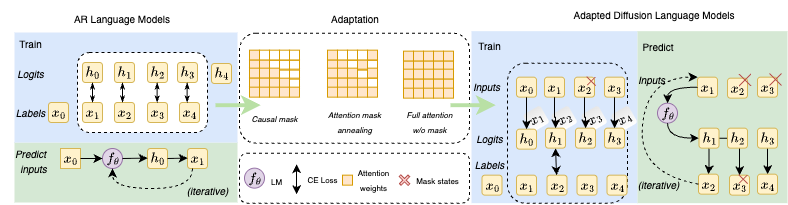
\includegraphics[width=0.95\textwidth]{figs/Adaptation/adaptation.png}
    \caption[Adaptation of AR models to diffusion models]{%
        The overview of Gong et al.'s~\cite{gong_scaling_2025} approach to adapt autoregressive (AR) models to diffusion models. 
        \textbf{Left}: The shift operation in AR models enables the output layer $h_i$ to approximate the distribution of next tokens $x_{i+1}$ in hidden representations through the cross entropy (CE) loss. 
        \textbf{Middle}: Gradually removing the causal mask during training eventually makes the model bidirectional. 
        \textbf{Right}: Inside the diffusion models, shifting the logits to compute the loss with the next token (i.e., the loss on $h_i$ would be concerning $x_{i+1}$), while perceptually, the diffusion models are still functioning as recovering the original signals (since $h_i$ corresponds to $x_{i+1}$ in AR loss).%
    }
    \label{fig:adaptation_overview}
\end{figure*}

% 对于 DLLMs 训练,来自 AR 模型的知识迁移可以作为缓解其历史较短和投资少于 AR 对应物的手段
For DLLM training, knowledge transfer from AR models can mitigate the challenges arising from their shorter development history and reduced investment compared to their AR counterparts. % DLLMs 可以从 AR 模型中蒸馏,就像较小的 AR 模型从较大的模型中逐令牌蒸馏一样
DLLMs can be distilled from AR models using the same token-by-token approach employed when distilling smaller AR models from larger ones. % Gong 等人在《通过自回归模型适应扩展扩散语言模型》中表明
Gong et al. present a method to in \textbf{Scaling Diffusion Language Models via Adaptation from Autoregressive Models}. Their approach first initializes the diffusion model's noise schedule and attention masks based on a pretrained AR checkpoint. Then the model is then fine-tuned with a combination of denoising and next-token prediction losses. The resulting DLLM inherits both the global coherence and fast convergence properties of the teacher AR model while retaining the parallel sampling advantages of diffusion. \cite{gong_scaling_2025}. % 具体来说,在适应训练期间,作者采用注意力掩码退火、移位操作和时间嵌入自由架构来缩小 AR 和 DLLMs 之间的差异
Specifically, during adaptation training, the authors employ attention mask annealing, shift operations, and a time‑embedding‑free architecture to reduce the gap between AR and DLLMs. \ref{alg:training} % 在采样期间,x_T 用所有掩码令牌初始化,然后基于时间反转分布采样令牌
During sampling, $\bm{x}_T$ is initialized with all \mask ~tokens, and tokens are subsequently sampled based on the time-reversal distribution $q(\bm{x}_s|\bm{x}_t, \bm{x}_0)$ \ref{alg:sampling}. The final loss at step $t$ is computed as:
\begin{equation}
% \textstyle
\label{eq:dm-loss}
    \mathcal{L}_{t}^{1:N} = \frac{1}{t}\mathbb{E}_{q(\mathbf{x}_t|\mathbf{x}_0)}\left[-\sum_{n=1}^N\delta_{\mathbf{x}_t^n,\bm{m}}(\mathbf{x}_0^{n})^\top\log f_{\theta}(\mathbf{x}_t^{1:N})_n\right],
\end{equation}%
where $\delta_{x_t^n, m}$ is the indicator function that equals 1 when $x_t^n = m$ (mask token) and 0 otherwise, and $f_\theta(x_t^{1:N})_n$ represents the model output of the $n$-th position of the sequence. For the sampling process, the backward transition distribution conditional on $\bm{x}_0$ is defined as: 
\begin{align}
\label{eq:qxs}
    q(\bm{x}_s|\bm{x}_t, \bm{x}_0) &= \frac{q(\bm{x}_t|\bm{x}_s)q(\bm{x}_s|\bm{x}_0)}{q(\bm{x}_t|\bm{x}_0)} \nonumber \\
    &= \begin{cases}
        \frac{\alpha_s-\alpha_t}{1-\alpha_t}\bm{x}_0+\frac{1-\alpha_s}{1-\alpha_t}\bm{m} & \text{if } \bm{x}_t=\bm{m}, \\
        \bm{x}_0 & \text{if }\bm{x}_t\neq\bm{m}.
    \end{cases}
\end{align}

\begin{algorithm}[H]
\footnotesize
\caption{Adaptation Training (Reproduced from \cite{gong_scaling_2025})}
\label{alg:training}
\begin{algorithmic}[1]
\State \textbf{Input:} network $f_{\theta}$ initialized by existing models, training corpus $p_{data}(\bm{x}_{0}^{1:N})$, mask token $\bm{m}$
\State \textbf{Output:} model parameters $\theta$
\Repeat
    \State Draw $\bm{x}_{0}^{1:N}\sim p_{data}$ and set \textit{labels} $\gets \bm{x}_{0}^{1:N}$
    \State Sample $t \sim \text{Uniform}(0,1)$
    \State Sample $\bm{x}_{t}^{1:N} \sim q(\bm{x}_{t}|\bm{x}_{0})$
    \State Anneal the attention mask \texttt{attn\_mask}
    \State Forward pass: \textit{logits} $\gets f_{\theta}(\bm{x}_{t}^{1:N})$ with \texttt{attn\_mask}
    \State Right shift \textit{logits} by one position \Comment{see Eq.~\ref{eq:dm-loss}}
    \State $\mathcal{L}_t = \frac{1}{t} \delta_{x_t, m} \cdot \text{CE}(\textit{logits}, \textit{labels})$
    \State Backpropagate using $\mathcal{L}_t$ and update $\theta$
\Until{convergence}
\end{algorithmic}
\end{algorithm}
Sampling strategies are central to the trade‐off between quality, speed, and stability in diffusion‐based text generation. In \textbf{energy‐based diffusion models}, a pretrained autoregressive (AR) model serves as an energy function to reweight samples drawn from the diffusion proposal distribution. The method restricts the importance sampling to a window of late diffusion timesteps and significantly reduces parallel decoding error. It enables high-fidelity outputs with significantly fewer denoising iterations, thereby reducing overall wall-clock time. Complete MCMC sampling remains infeasible in the high-dimensional token space. Therefore, importance sampling remains the preferred alternative \cite {xu_energy-based_2025}.  



Furthermore, masked diffusion models can accelerate inference by skipping redundant noise levels. In “\textbf{Simple and Effective Masked Diffusion Language Models},” the authors introduce an \textbf{Efficient Ancestral Sampling} scheme that dynamically omits specific intermediate timestamps during denoising, reducing the number of functional calls to the denoiser without degrading output quality \cite{sahoo_simple_2024}.  



Recently, the \textbf{Large Language Diffusion Models (LLaDA)} framework employs two complementary remasking strategies to concentrate computation on uncertain tokens. First, \emph{low‐confidence remasking} re‐noises only those tokens whose predicted confidence falls below a threshold, focusing denoising steps where they matter most. Second, a \emph{semi‐autoregressive remasking} divides the sequence into blocks that are generated left‐to‐right but sampled in parallel within each block, achieving a balance between sequential coherence and parallel throughput \cite{nie_large_2025}.  



Generalized Interpolating Discrete Diffusion (GIDD) adds a self‐correction iteration after full denoising: the model resamples tokens based on its likelihood estimates, committing the highest‐scoring changes until convergence. The fixed-point refinement step mitigates error propagation from early timesteps, thus yields more coherent sequences without requiring additional training \cite {rutte_generalized_2025}.  



To sum up, these sampling innovations: importance sampling windows, efficient ancestral skipping, confidence-based remasking, and self-correction demonstrate the careful scheduler and sampler design can significantly improve both the speed and quality of diffusion-based text generation.  



% \bibliographystyle{plain}

% \bibliography{DLLM}



% 基于能量的扩散提供了第二种蒸馏模式
Energy based diffusion offers an alternative distillation approach: % Xu 等人证明通过使用预训练的 AR 模型作为扩散框架中的能量函数
Xu \emph{et al.} demonstrate that by employing a pretrained AR model as the energy function within a diffusion framework, one effectively distills the AR model's token probabilities into a diffusion proposal distribution. % 在推理时,从扩散模型并行采样的样本通过 AR 能量重新加权或重新评分
At inference time, samples drawn in parallel from the diffusion model are reweighted or rescored by the AR energy function, correcting decoding errors and achieving AR level quality with substantially fewer sequential steps \cite{xu_energy-based_2025}.

% 这些蒸馏技术还增强了推测解码
These distillation techniques also enhance speculative decoding: when the diffusion draft model has been distilled from an AR teacher, its proposals during speculative sampling exhibit significantly higher accuracy, resulting in reduced rejection rates and improved overall throughput compared to undistilled drafts \cite{christopher_speculative_2025}.

% 相反,AR 模型可以吸收扩散风格的表示
Conversely, AR models can incorporate diffusion style representations. % Lovelace 等人重新利用预训练 AR 模型的编码器-解码器潜在空间
Lovelace \emph{et al.} repurpose the encoder-decoder latent space of a pretrained AR model to learn a high-dimensional diffusion process that captures token-to-token correlations beyond the standard AR factorization. % 通过在 AR 解码循环中交错基于扩散的潜在细化步骤
By interleaving diffusion-based latent refinement steps within the AR decoding loop, the hybrid system achieves superior diversity and controllability while maintaining AR fluency \cite{lovelace_latent_2023}.

% 这些工作共同建立了双向桥梁
Together, these research directions establish a bidirectional bridge: % AR 模型可以通过蒸馏为高效的 DLLM 训练提供种子和指导
AR models can seed and guide efficient DLLM training through distillation, % 而 DLLM 机制可以通过并行细化阶段丰富 AR 解码器
while DLLM mechanisms can enrich AR decoders with parallel refinement capabilities. % 这种归纳偏置的相互迁移有望产生融合两种范式优势的新混合架构
This mutual transfer of inductive biases promises novel hybrid architectures that effectively combine the strengths of both paradigms.

% \bibliographystyle{plain}
% \bibliography{DLLM}




% Collaboration
\section{Collaboration between Diffusion-based and Autoregressive Models at Inference Time}
\label{sec:collaboration}
Recent work has shown that diffusion-based language models (DLLMs) and autoregressive (AR) models can be combined in complementary ways to leverage the strengths of both paradigms. For example, HybridVLA interleaves an AR component for text and image generation with a diffusion component operating on the action space of an embodied agent, allowing a single model to generate rich multimodal descriptions and execute coherent action plans \cite{liu_hybridvla_2025}. In \textbf{Block Diffusion}, fixed-size blocks of tokens are generated by first sampling the initial token autoregressively, then denoising the remainder of the block in parallel via a DLLM, achieving a balance between sequential decoding speed and parallel sampling efficiency \cite{arriola_block_2025}.  

\noindent\textbf{DiffPO} applies a diffusion-style denoising step at inference time to align AR-generated sentences with learned human ``preference'' vectors, reshaping outputs post hoc without retraining the underlying AR model and improving both fluency and alignment metrics \cite{chen_diffpo_2025}. Similarly, Latent Diffusion for Language Generation projects token embeddings into a compact latent space via a compression network and reconstructs tokens through an AR decoder, speeding up sampling while preserving generation quality \cite{lovelace_latent_2023}.  

\noindent In an energy-based approach, \textbf{Energy-Based Diffusion Language Models} train a diffusion process to match a target AR distribution, enabling ``plug and play'' sampling from pretrained AR models via energy gradients and bridging sample efficiency with expressive power \cite{xu_energy-based_2025}. Building on this idea, Speculative Diffusion Decoding uses a fast DLLM as a draft generator to propose multiple continuations in parallel, which are then scored or filtered by an AR model to achieve near AR quality with fewer sequential steps \cite{christopher_speculative_2025}.  

\noindent \textbf{DDPT: Diffusion-Driven Prompt Tuning} uses a DLLM to generate or refine prompts in latent space for a large language model focused on code generation; the prompt is then passed to an AR code generator, and the overall loss computed against ground truth code tunes the prompt space via diffusion \cite{li_ddpt_2025}. On the theoretical side, a \textbf{Unified Hyperschedules Framework} demonstrates that autoregression arises as a special case of diffusion under extreme noise schedules; by modulating noise levels and step counts, one can smoothly interpolate between pure AR and diffusion, or combine them to harness both methods' advantages \cite{fathi_unifying_2025}.  

\noindent \textbf{TEncDM} operates diffusion not on raw tokens but in the continuous encoding space of a frozen LLM encoder–decoder, using cross attention for self-conditioning. This leverages powerful transformer representations while accelerating refinement through parallel diffusion sampling \cite{shabalin_tencdm_2025}.  

\begin{figure}[h!]
    \centering
    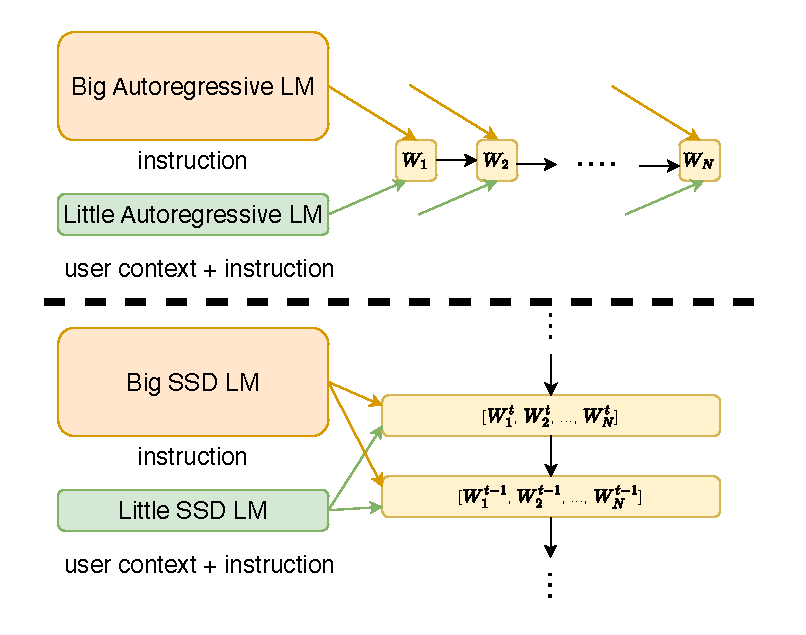
\includegraphics[width=0.5\textwidth]{figs/David_helps_Goliath.pdf}
    \caption[\textit{David helps Goliath} collaboration framework]{%
        \textit{David helps Goliath}~\cite{han_david_2024}: Inference-time collaboration between large and small models. 
        AR models decode token-by-token, while diffusion models refine token blocks iteratively with bidirectional contexts.%
    }
    \label{fig:david_helps_goliath}
\end{figure}

\noindent Finally, \textbf{David helps Goliath} demonstrates DLLM's mutual collaboration advantage over autoregressive counterparts: DLLMs' iterative generation process enables them to reference bidirectional context, therefore, it is easier for different DLLMs to collaborate at the sequence level and yield better quality. Inspired by AR counterparts, the authors incorporate the logits-averaging method to generate a block of tokens at each diffusion step for expert model $\theta_{\mathrm{core}}$ and user model $\theta_{\mathrm{user}}$. Similar to AR counterparts, to increase the pointwise information exchange between the expert generated data and the conditioned generation based on the instruction, a contrastive term $\theta_{\mathrm{user}}$ without input $D_{\text{user}}$ is added.\cite{han_david_2024}

%\begin{equation}
%\label{eq:david_helps_goliath}
%\footnotesize
\small
\begin{align*}
    \boldsymbol{w}_{\text{core-logits}, t}^{c:c+B} &= \operatorname{logits}_{\theta_{\text{core}}}(\boldsymbol{w}^{c:c+B} \mid \boldsymbol{w}_{\text{inst}}, \boldsymbol{w}^{<c}, \Tilde{\boldsymbol{w}}_t^{c:c+B}) \\
    \boldsymbol{w}_{\text{user-logits}, t}^{c:c+B} &= \operatorname{logits}_{\theta_{\text{user}}}(\boldsymbol{w}^{c:c+B} \mid D_{\text{user}}, \boldsymbol{w}_{\text{inst}}, \boldsymbol{w}^{<c}, \Tilde{\boldsymbol{w}}_t^{c:c+B}) \\
    \boldsymbol{w}_{\neg \text{user-logits}, t}^{c:c+B} &= \operatorname{logits}_{\theta_{\text{user}}}(\boldsymbol{w}^{c:c+B} \mid \boldsymbol{w}_{\text{inst}}, \boldsymbol{w}^{<c}, \Tilde{\boldsymbol{w}}_t^{c:c+B}) \\
    \boldsymbol{w}_{\text{logits}, t}^{c:c+B} &= (1-\lambda_{\text{user}}) \boldsymbol{w}_{\text{core-logits}, t}^{c:c+B} \\
    &\quad + \lambda_{\text{user}} (1+\alpha) \boldsymbol{w}_{\text{user-logits}, t}^{c:c+B} - \lambda_{\text{user}} \alpha \boldsymbol{w}_{\neg \text{user-logits}, t}^{c:c+B}
\end{align*}
%\end{equation}


\noindent Together, these approaches illustrate a rich design space for hybrid generation: blockwise and latent space diffusion, post-hoc preference alignment, speculative drafting, prompt tuning, and unified theoretical frameworks. All pointing toward future models that fluidly integrate diffusion and autoregression within a single system.






\section{Inference Speed of Diffusion Language Models}
\label{sec:inference_speed}


In David helps Goliath, the authors find the generation no longer updates for the last 40\% of the inference time. They incorporate an early-stop strategy: halting the small model from generation based on empirically determined time range: \textit{t = 0.4T}, the pipeline reduces the total number of denoising steps by 40\% without sacrificing output quality. \cite{han_david_2024} 

Building on ideas from autoregressive speculative decoding, Speculative Diffusion Decoding uses a fast DLLM as a draft generator and an AR model as the verifier. The diffusion draft draws $k$ tokens in parallel and the AR target then confirms or corrects them, yielding substantial speedups even without fine-tuning the diffusion draft \cite{christopher_speculative_2025}. This two-stage process highlights how parallel sampling can be combined with selective sequential verification to accelerate decoding.

Self-conditioned discrete diffusion processes can match autoregressive latency through parallel sampling. In their work on \textbf{SEDD}, Lou \emph{et al.} demonstrate that around 100 denoising steps suffice to match AR inference time, and by removing KV-cache dependencies, throughput can increase by 4–6× \cite{lou_discrete_2024}. This result highlights the potential of batch parallelism and cache-free sampling in reducing the speed gap between diffusion and autoregressive models.

Task-specific optimizations also yield notable gains. The \textbf{Discrete Diffusion Language Model for Efficient Text Summarization} employs tailored noise schedules and reduced-step denoising to outperform both AR and continuous-diffusion baselines on wall-clock decoding time \cite{dat_discrete_2025}. By focusing computation on the most informative tokens, the efficiency of summarization is greatly enhanced.

Reparameterization of discrete diffusion versus continuous dynamics has a significant impact on convergence speed. Zheng \emph{et al.} analyze how continuous diffusion over token embeddings converges slowly—meaningful tokens only emerge after hundreds or thousands of iterations—while reparameterized discrete diffusion achieves coherent text generation in tens of steps, explaining much of the observed speed disparity \cite{zheng_reparameterized_2024}.

In Energy-Based Diffusion Language Models, a pretrained AR model serves as an energy function within the diffusion sampler. By applying importance sampling on late timesteps, required denoising steps can be reduced while maintaining AR-level generation quality under the same latency budget \cite{xu_energy-based_2025}. This approach illustrates how energy-based rejection sampling can accelerate diffusion inference.

Finally, \textbf{Your Absorbing Discrete Diffusion} removes time-conditioning in its Markov kernel to enable KV-style caching of intermediate predictions, further speeding up sampling compared to standard absorbing diffusion formulations \cite{ou_your_2025}. This caching mechanism highlights how architectural modifications can alleviate the overhead of iterative denoising.

\begin{figure*}[ht]
    \centering
    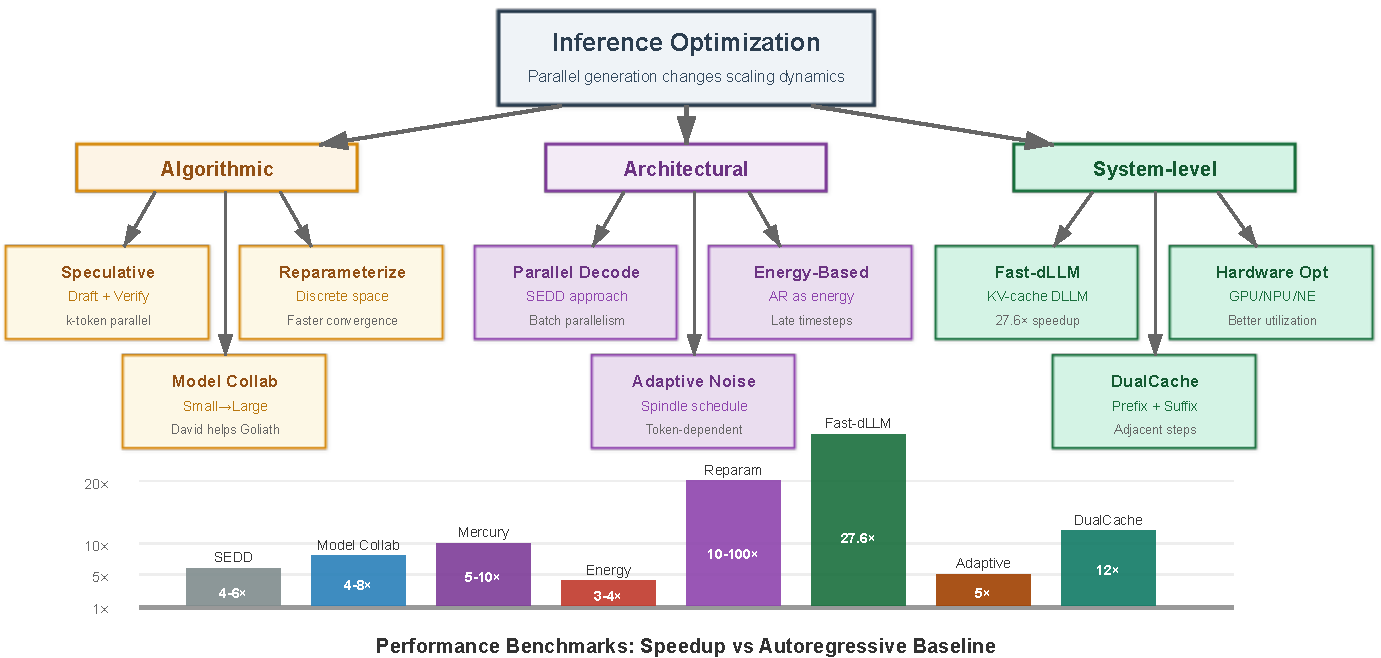
\includegraphics[width=1.0\textwidth]{figs/8_inference_speed.pdf}
    \caption{DLLM Inference Speed Optimization Techniques}
    \label{fig:dllm_inference_speed}
\end{figure*}

% \bibliographystyle{plain}
% \bibliography{DLLM}

\section{Impact of Sampling Techniques on Performance}
\label{sec:sampling}
Sampling strategies are central to the trade‐off between quality, speed, and stability in diffusion‐based text generation. In \textbf{energy‐based diffusion models}, a pretrained autoregressive (AR) model serves as an energy function to reweight samples drawn from the diffusion proposal distribution. The method restricts the importance sampling to a window of late diffusion timesteps and significantly reduces parallel decoding error. It enables high-fidelity outputs with significantly fewer denoising iterations, thereby reducing overall wall-clock time. Complete MCMC sampling remains infeasible in the high-dimensional token space. Therefore, importance sampling remains the preferred alternative \cite {xu_energy-based_2025}.  



Furthermore, masked diffusion models can accelerate inference by skipping redundant noise levels. In “\textbf{Simple and Effective Masked Diffusion Language Models},” the authors introduce an \textbf{Efficient Ancestral Sampling} scheme that dynamically omits specific intermediate timestamps during denoising, reducing the number of functional calls to the denoiser without degrading output quality \cite{sahoo_simple_2024}.  



Recently, the \textbf{Large Language Diffusion Models (LLaDA)} framework employs two complementary remasking strategies to concentrate computation on uncertain tokens. First, \emph{low‐confidence remasking} re‐noises only those tokens whose predicted confidence falls below a threshold, focusing denoising steps where they matter most. Second, a \emph{semi‐autoregressive remasking} divides the sequence into blocks that are generated left‐to‐right but sampled in parallel within each block, achieving a balance between sequential coherence and parallel throughput \cite{nie_large_2025}.  



Generalized Interpolating Discrete Diffusion (GIDD) adds a self‐correction iteration after full denoising: the model resamples tokens based on its likelihood estimates, committing the highest‐scoring changes until convergence. The fixed-point refinement step mitigates error propagation from early timesteps, thus yields more coherent sequences without requiring additional training \cite {rutte_generalized_2025}.  



To sum up, these sampling innovations: importance sampling windows, efficient ancestral skipping, confidence-based remasking, and self-correction demonstrate the careful scheduler and sampler design can significantly improve both the speed and quality of diffusion-based text generation.  



% \bibliographystyle{plain}

% \bibliography{DLLM}


%%%%


\section{Fine-Tuning of Diffusion Language Models}
\label{sec:finetuning}
Fine-tuning diffusion language models (DLLMs) extends their flexibility and task adaptability, drawing inspiration from autoregressive (AR) LLM fine-tuning techniques. Recent work demonstrates several viable pathways.

In David helps goliath, the authors report one of the first instances of DLLM fine-tuning by leveraging the DOLLY dataset (15K human-collected instructions and responses) to adapt their SSD-2 diffusion model for downstream tasks. The authors show the finetuned model is better at collaboration than autoregressive counterpart thanks to the bidirectional context reference during ensemble \cite{han_david_2024}.

The \textbf{Mercury Diffusion Language Model} technical report explores alignment-focused fine-tuning strategies: reinforcement learning from human feedback (RLHF) and direct preference optimization (DPO) have been used to guide the diffusion denoiser towards preferred outputs.  By integrating these feedback signals at inference-time trajectories, the model rapidly aligns to user-specified functions, suggesting that DLLMs can match or exceed AR alignment speed \cite{labs2025mercuryultrafastlanguagemodels}.

Supervised fine-tuning (SFT) also proves effective. In Large Language Diffusion Models (LLaDA), the authors demonstrate conventional instruction-driven SFT on a diffusion backbone, showing scalable improvements in generative accuracy across a range of tasks.  By framing instructions as conditioning masks in the denoising process, DLLMs achieve comparable zero-shot performance to AR LLMs post-finetuning \cite{nie_large_2025}.

Beyond standard SFT, Instruction Fine-Tuning further enhances generalization.  \textbf{Diffusion Language Models Can Perform Many Tasks with Scaling and Instruction-Finetuning} shows instruction-tuned diffusion models generalize to unseen languages and tasks without additional data. E.g., German text generation emerges zero-shot after English only fine-tuning and highlighting the strong transfer capacity of DLLMs \cite{ye_diffusion_2025}.

These studies reveal a promising interpolation between AR and diffusion fine-tuning. Parameter-efficient adapters and instruction masks can be seamlessly adapted to the denoising architecture; this enables rapid specialization and alignment.  Potential future work includes integrating LoRA - low-rank adaptation techniques to reduce tuning overhead and explore hybrid schedules that jointly adjust AR and diffusion components during fine-tuning.

\begin{figure*}[ht]
    \centering
    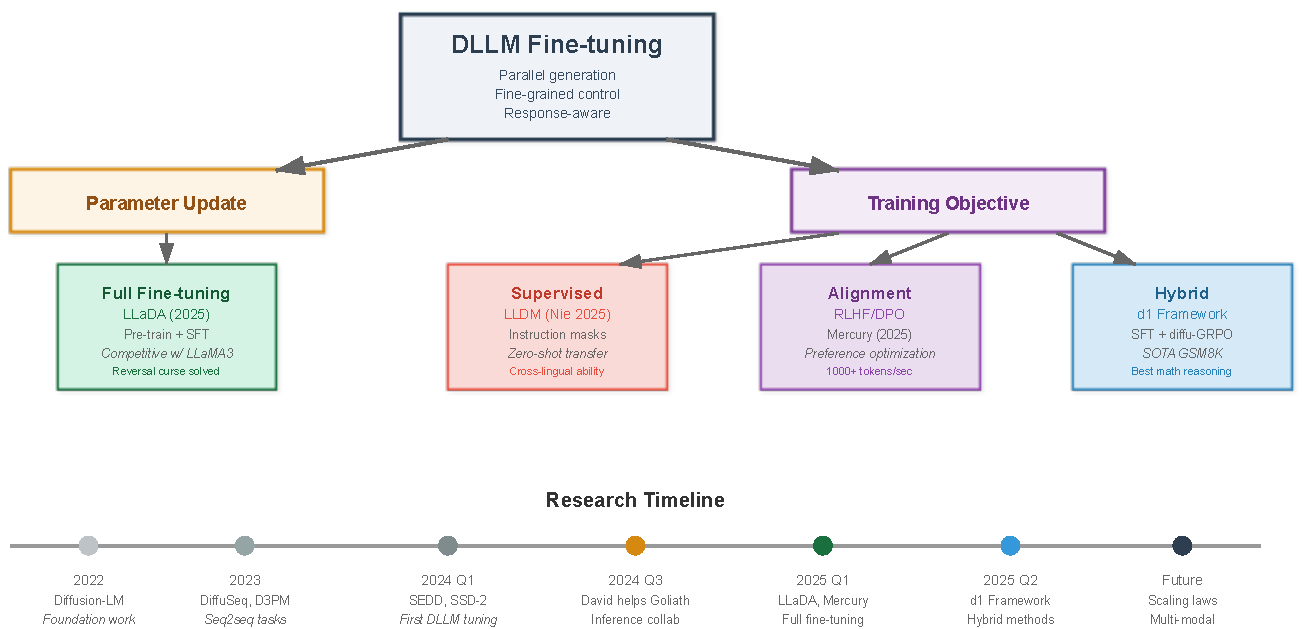
\includegraphics[width=0.9\textwidth]{figs/10_finetune.pdf}
    \caption{DLLM Fine-tuning Methods: Taxonomy and Evolution}
    \label{fig:dllm_finetune}
\end{figure*}

% \bibliographystyle{plain}
% \bibliography{DLLM}

\section{Multimodality and Reasoning Capabilities of Diffusion Language Models}
\label{sec:frontier}
Recent work has begun to expand diffusion language models (DLLMs) beyond pure text generation into the realms of multimodal understanding and complex reasoning. In the multimodal domain, Diffusion Language Models Can Perform Many Tasks with Scaling and Instruction-Finetuning demonstrates that a single discrete-diffusion backbone can be extended to process image inputs and answer visual questions. By following the two-phase training paradigm of LLaVA—first interleaving visual and textual encodings in a frozen vision encoder, then instruction-fine-tuning the diffusion decoder—DLLMs attain zero-shot performance on vision-language benchmarks without specialized cross-modal architectures \cite{ye_diffusion_2025}. This result highlights DLLMs’ ability to treat images as another “language” of tokens, leveraging the random-masking denoising process to fuse visual and linguistic representations seamlessly.

On the reasoning front, \textbf{d1: Scaling Reasoning in Diffusion Large Language Models via Reinforcement Learning} introduces a two-stage post-training framework—supervised fine-tuning on high-quality reasoning traces followed by a novel policy gradient method (\textbf{diffu-GRPO})—to imbue masked DLLMs with stepwise planning capabilities. Remarkably, as sequence lengths exceed 512 tokens, the model begins to exhibit self-correction and backtracking behaviors, mirroring the “chain-of-thought” processes seen in autoregressive counterparts, yet without relying on a fixed generation order. Furthermore, instruction-fine-tuned DLLMs are shown to conform their generative steps to a topological sort of the underlying causal graph—first generating premises, then formulas, then conclusions—underscoring their inherent advantage in modeling non-linear dependencies over unidirectional AR decoders \cite{zhao_d1_2025}.

The key innovation of \textbf{d1} lies in adapting Group Relative Policy Optimization (GRPO) for the DLLM's architecture. Traditional policy gradient methods encounter challenges here due to DLLMs non-autoregressive nature. To address this, the authors develop diffu-GRPO, which modifies the standard GRPO objective to handle partially masked sequences. To compute the log-probability of each token $o$ in the sequence in the diffu-GRPO framework, for a given prompt $q$, a perturb process is executed on it where each token randomly gets masked with probability $p_{\text{mask}}$, generating a masked prompt $q'$. Then a one step unmasking process is executed to obtain the estimation of per-token log-probability $\log \pi_\theta(o^k | q)$, $1\leq k \leq |o|$. The advantage for token $k$ in response $o_i$ is computed using the group-relative approach: 
\begin{equation}
A_i^k(\pi) = r_i(\pi) - \text{mean}\left(\{r_j(\pi)\}_{j=1}^G\right), \quad 1 \leq k \leq |o_i|,
\label{eq:grpo-advantage}
\end{equation}%
where $r_i(\pi)$ represents the reward for response $i$, and $G$ is the total number of responses sampled from the current policy. The optimization objective combines this advantage calculation with policy gradient updates specifically designed for masked sequences. The diffu-GRPO loss function incorporates both the policy improvement term and KL divergence regularization:
\begin{equation}
\begin{aligned}
\mathcal{L}_{\text{diffu-GRPO}}(\theta) &= \mathbb{E}_{\substack{q \sim \mathcal{D},\, q' \sim \text{masking}(q),\\
              o_1,\dots,o_G \sim \pi_{\theta_{\text{old}}}(\,\cdot \mid q)}}\Bigg[
\frac{1}{G}\sum_{i=1}^{G}\frac{1}{|o_i|}\sum_{k=1}^{|o_i|}\\
&\quad\min\!\Bigg(
      \frac{\phi^{\pi_\theta}(o^k_i \mid q')}
           {\phi^{\pi_{\theta_{\text{old}}}}(o^k_i \mid q')}A_i^{k},\\
&\qquad\operatorname{clip}\!\Bigg(
        \frac{\phi^{\pi_\theta}(o^k_i \mid q')}
             {\phi^{\pi_{\theta_{\text{old}}}}(o^k_i \mid q')},
        1-\varepsilon,\,1+\varepsilon
  \Bigg)A_i^{k}
\Bigg)\\
&\quad-\beta\,D_{\text{KL}}\!\Bigl[
   \phi^{\pi_\theta}(\cdot \mid q')\,\bigl\|\,\phi^{\pi_{\text{ref}}}(\cdot \mid q')
\Bigr]
\Bigg],
\end{aligned}
\label{eq:diffugrpo}
\end{equation}%
where $\phi^{\pi_\theta}(o^k \mid q')$ and $\phi^{\pi_\theta}(o \mid q')$  denote the estimated per-token and sequence probabilities for $\pi_\theta$, and $\beta$ controls the strength of the KL divergence penalty. The algorithm of diffu-GRPO is summarized in Algorithm~\ref{alg:diffu-grpo}.

\begin{algorithm}[t]
\footnotesize
\caption{diffu-GRPO: Policy Gradient Optimization for Masked dLLMs (Reproduced from d1~\cite{zhao_d1_2025})}
\label{alg:diffu-grpo}
\begin{algorithmic}[1]
\State \textbf{Require:} Reference model $\pi_{\text{ref}}$, prompt distribution $\mathcal{D}$, number of completions per prompt $G$, number of inner updates $\mu$, prompt token masking probability $p_{\text{mask}}$
\State \textbf{Initialize} $\pi_\theta \leftarrow \pi_{\text{ref}}$
\While{not converged}
    \State $\pi_{\text{old}} \leftarrow \pi_\theta$
    \State Sample a prompt $q \sim \mathcal{D}$
    \State Sample $G$ completions $o_i \sim \pi_{\theta_{\text{old}}}(\cdot | q)$, $i \in [G]$\
    \State For each $o_i$, compute reward $r_i$ and advantage $A_i^k(\pi_{\theta_{\text{old}}})$ using Eq.~\ref{eq:grpo-advantage}
    \For{gradient update iterations $n = 1, \ldots, \mu$}
        \State $q' \leftarrow$ randomly mask tokens of prompt $p$ with probability $p_{\text{mask}}$
        \State For $\pi_\theta, \pi_{\theta_{\text{old}}}, \pi_{\text{ref}}$, estimate log-probabilities of $o_i$ given $q'$ 
        \State Compute diffu-GRPO objective (\ref{eq:diffugrpo}) and update $\pi_\theta$ by gradient descent
    \EndFor
\EndWhile
\State \Return $\pi_\theta$
\end{algorithmic}
\end{algorithm}

By abstracting both images and complex logical steps as masked tokens in a unified diffusion process, these frontier studies reveal that DLLMs can serve as generalist engines for multimodal perception and multi-step reasoning. Future work will undoubtedly refine these training recipes and explore more modality integrations and "knowledge transfer" of different modalities between AR models and DLLMs.

\begin{figure*}[ht]
    {\centering
    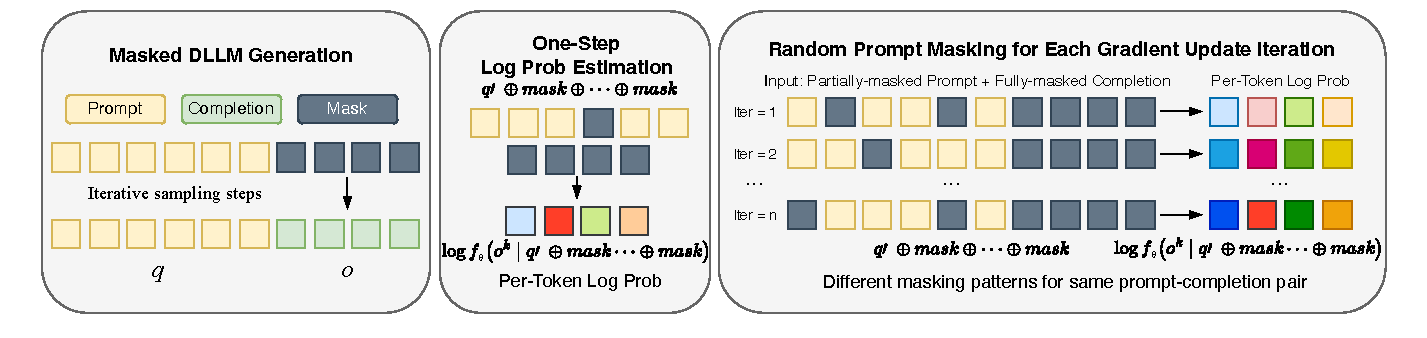
\includegraphics[width=1.0\textwidth]{figs/diffu_grpo.pdf}
    \par}
    \caption{\textbf{Log Probability Estimation in diffu-GRPO.} First the completion $o$ is generated from prompt $q$ using full diffusion sampling \textbf{(left)}. Then token-level log probabilities are computed using a single forward pass for each masking pattern \textbf{(mid)}. The log-probability from one-step unmasking is used as the estimation method. During policy gradient updates, a random masking pattern is applied to the prompt to create $q'$, while the completion stays fully masked \textbf{(right)}. The color gradients in per-token log probabilities show that different masking patterns give different estimates of token-level log probabilities. This works as a regularization method for policy optimization, allowing more gradient updates per batch. This approach reduces the number of online generations needed for RL training.}
    \label{fig:diffu-GRPO}
\end{figure*}

% \bibliographystyle{plain}
% \bibliography{DLLM}




\section{Evaluation of Diffusion Language Models}
\label{sec:evaluation}
Evaluating diffusion language models (DLLMs) requires metrics that capture both generative quality and the distinctive inference characteristics of diffusion processes. We discuss common benchmarks and their limitations when applied to DLLMs.



\noindent\textbf{Language modeling.}  To compare token prediction accuracy with autoregressive (AR) baselines, DLLMs often report perplexity on datasets like WikiText-103 and Penn Treebank.  For example, Block Diffusion and Reparameterized discrete models approach AR perplexity after sufficient training steps \cite{arriola_block_2025, zheng_reparameterized_2024}.  However, perplexity assumes a left-to-right factorization and ignores DLLM’s parallel sampling and iterative refinement. This potentially underestimates diffusion models optimized for inference speed.  Complementary metrics such as BERTScore have been proposed to evaluate contextual similarity beyond token-level likelihood \cite{zhang_bertscore_2019}, yet these do not reflect generation latency.



\noindent\textbf{Sequence-to-sequence tasks.}  Machine translation and summarization evaluations use BLEU and ROUGE scores on WMT and CNN/DailyMail benchmarks \cite{papineni_bleu_2002, lin_rouge_2004}.  Discrete Diffusion for Summarization achieves ROUGE comparable to AR systems with fewer denoising steps \cite{dat_discrete_2025}. Besides, COMET provides a learned evaluation that correlates better with human judgments on translation \cite{rei_comet_2020}.  Diversity metrics such as distinct-n and Self-BLEU quantify the variety of generated outputs, which is important for diffusion modelsparallel proposals \cite{li_diversity_2016}.



\noindent\textbf{Open-ended generation.}  Distributional metrics such as MAUVE measure the divergence between model and human text distributions \cite{pillutla_mauve_2021}. Meanwhile, diversity measures (distinct-1/2) assess intra-sample variety.  MAUVE better reflects human preference than perplexity, but it overlooks diffusion’s multi-step denoising trajectories and interactive editing capabilities.  Human evaluations, preferences or side-by-side comparisons, are still essential yet are infrequent due to cost.



\noindent\textbf{Reasoning and instruction following.}  Benchmarks, such as GSM8K, CommonsenseQA, and StrategyQA assess multi-step and commonsense reasoning.  Instruction-fine-tuned DLLMs demonstrate zero-shot performance on unseen tasks, matching AR LLMs in reasoning accuracy \cite{zhao_d1_2025}. BigBench Hard tasks reveal areas where diffusion planning may excel \cite{srivastava_bigbench_2022}.  However, some reasoning benchmarks focus on final answers and ignore DLLM’s intermediate planning and self-correction behaviors.



\noindent\textbf{Multimodal and embodied tasks.}  Models such as HybridVLA are evaluated on VQA accuracy, COCO caption CIDEr, METEOR, and SPICE scores \cite{liu_hybridvla_2025, anderson_spice_2016}.  Although, these benchmarks test cross-modal alignment, they do not capture DLLM’s capacity for iterative visual refinement or privacy-preserving on-device drafts.



\noindent\textbf{Robustness and calibration.}  Adversarial and stress tests—e.g.\ perturbed prompts or style shifts, measure model stability under input variation \cite{eger_robustness_2021}.  Calibration metrics such as expected calibration error (ECE) evaluate confidence alignment, relevant for diffusion’s energy-based sampling, however it is rarely reported \cite{guo_calibration_2017}.



\noindent\textbf{Inference speed and efficiency.} Real-world evaluation should include wall-clock latency and throughput.  Self-Conditioned Discrete Diffusion (SEDD) matches AR latency at ~100 steps and attains 4–6× higher batch throughput by removing KV-cache dependencies \cite{lou_discrete_2024}.  Energy-based importance sampling reduces denoising iterations, achieving AR-level quality under the same time budget \cite{xu_energy-based_2025}.  Most DLLM works, however, still report only step counts rather than end-to-end latency metrics.



While perplexity, BLEU/ROUGE, MAUVE, and other distributional or learned metrics offer useful baselines, they often underrepresent diffusion’s parallelism, controllability, and iterative refinement.  We advocate for \emph{latency-aware} benchmarks, \emph{intermediate-step quality tracking}, and \emph{interactive tasks} that leverage self-correction and multi-token proposals to fully characterize DLLM capabilities.




\section{Applications of Diffusion Language Models}
\label{sec:applications}
Diffusion language models (DLLMs) have grown beyond simple text generation. When we regard specialized data—such as protein sequences, molecular graphs, or genomic DNA—as distinct “languages,” DLLMs demonstrate remarkable versatility across both scientific and multimodal fields.


In \textbf{text-to-video} generation, researchers have successfully combined large language models with diffusion priors to generate videos base on the natural-language instructions. For example, in “The Best of Both Worlds: Integrating Language Models and Diffusion Models for Video Generation,” the authors show how prompt-conditioned diffusion transformers can generate successive frames that remain temporally consistent and closely aligned with the user’s text prompt \cite{yin_best_2025}.


DLLMs have also been applied to \textbf{protein and molecule design}. In \textbf{DiffSDS}, protein backbone inpainting is formulated as a masked diffusion process over torsion angles.  This enables the model to complete structures accurately under defined geometric constraints \cite{gao_diffsds_2023}. DPLM‑2 employs two separate tokenizers—for amino‑acid sequences and structural motifs—and jointly denoises both representations to propose novel protein scaffolds \cite{wang_dplm-2_2024}. In the domain of small-molecule discovery, \textbf{Constrained Discrete Diffusion (CDD)} enforces chemical valence and substructure rules at every denoising iteration. The technique ensures that the generated compounds are both chemically valid and sufficiently novel for drug and materials research \cite{cardei_constrained_2025}.


Beyond proteins, DLLMs have been extended to \textbf{genomic sequence modeling}. Simple and Effective Masked Diffusion Language Models (MDLM) is a new way to generate text by gradually filling in masked words. It trains an encoder-only model with a mix of classic masked language losses, then samples text in a few semi-autoregressive steps. On benchmarks like LM1B and OpenWebText, MDLM cuts diffusion model perplexity close to standard autoregressive methods. \cite{sahoo_simple_2024}.


In \textbf{text summarization}, CrossMamba perform blockwise denoising over entire documents, achieving faster decoding speeds and better content preservation than typical autoregressive summarization on Gigaword andCNN/DailyMail datasets \cite{dat_discrete_2025}. Moreover, DLLM‑based classifiers can maintain an author’s original stance—particularly in political news—by applying preference‑guided denoising at inference time \cite{liu_p3sum_2024}.


The applications extend into \textbf{robotics}. The HybridVLA model fuses diffusion‑generated action plans with autoregressive textual descriptions, enabling an embodied agent to both plan and verbally explain its actions in a coherent manner \cite{liu_hybridvla_2025}.


For \textbf{privacy-sensitive inference}, the David helps Goliath framework partitions computation: a lightweight diffusion model operates locally on the user’s device and a remote expert model. The generation on the local diffusion model only defers to a remote expert model when necessary. In this way, user data remains confidential while the overall generative performance is preserved \cite{han_david_2024}.


DLLMs have further been adapted for \textbf{seq2seq} tasks, such as machine translation and data‑to‑text conversion, through DiffuSeq’s parallel masked denoising pipeline \cite{gong_diffuseq_2023}. In \textbf{alignment-based editing},methods like DiffPO apply targeted denoising to achieve controlled sentiment or stylistic transformation in text \cite{chen_diffpo_2025}. There are even emerging models for \textbf{sign language production}, where sequences of gesture tokens are generated from textual input using discrete diffusion processes \cite{he_text-driven_2025}.


By abstracting structured data as discrete languages, DLLMs unlock new possibilities in scientific discovery, multimedia creation, and human–machine interaction—showing that the same underlying principles can be tailored to a wide array of domains.



% \bibliographystyle{plain}



% \bibliography{DLLM}




\section{Future Research Directions}
\label{sec:future}
Despite that diffusion language models (DLLMs) have made great progress in text, multimodal, and scientific domains, several challenges and promising directions are yet to be explored.



Adaptive and budgeted sampling seem promising. Although Speculative Diffusion Decoding \cite{christopher_speculative_2025} and importance sampling windows in energy‐based samplers \cite{xu_energy-based_2025} yield speedups, DLLMs still rely on tens to hundreds of denoising steps. Future work may explore \textbf{learned noise schedules} that dynamically allocate iterations based on token uncertainty; implement \textbf{budgeted diffusion}, in which a global compute or latency budget enables early stopping. Continuous‐time samplers such as DDIM \cite{song_denoising_2020} that can execute sampling process with adaptive step-size control, may offer further acceleration while preserving sample quality.



Alignment and controllability remain another key issue. Initial alignment techniques: RLHF and DPO in the Mercury report \cite{labs2025mercuryultrafastlanguagemodels} and DiffPO~\cite{chen_diffpo_2025}, demonstrate feasibility on small models, but scaling to large diffusion architectures demands \textbf{parameter-efficient adapters} (e.g., LoRA) tailored for denoising networks. Moreover, integrating \textbf{classifier-free guidance} \cite{ho_classifier-free_2022} into diffusion samplers could enable fine-grained control without having external energy networks.



Hybrid diffusion–autoregressive paradigms can combine the strengths of both worlds. Block Diffusion \cite{arriola_block_2025} and \emph{TEncDM} \cite{shabalin_tencdm_2025} illustrate how AR and diffusion models cooperate. Future research may investigate \textbf{joint training objectives}, that blend maximum-likelihood AR losses with score-matching. Build on this, researchers may develop \textbf{mixture-of-sampling experts} that choose between AR and diffusion per token or block based on context and compute constraints.



Multimodal and structured generation are ripe for expansion. Building on HybridVLA \cite{liu_hybridvla_2025}, we see \textbf{modality-agnostic architectures} having the capability of unified text, vision, audio, and graph diffusion. In scientific domains, graph-structured diffusion processes for molecules \cite{rutte_generalized_2025} and proteins \cite{gao_diffsds_2023} can benefit from \textbf{self-correction} techniques exemplified by GIDD \cite{rutte_generalized_2025} to enforce structural validity.



The interactive nature of diffusion sampling suggests novel human-in-the-loop applications. \textbf{Live editing interfaces} can allow users to re-mask and refine tokens during generation,while \textbf{cascaded refinement pipelines} can progressively enhance outputs via coarse-to-fine diffusion stages. Such interactive paradigms can leverage DLLM’s parallel proposals for rapid user feedback.



Understanding and interpreting diffusion models across languages remains under explored. We encourage research about  \textbf{information-theoretic analyses}: how noise schedules impact modeling capacity and diversity. For theoretical work, researchers should focus on bridging diffusion and autoregression via the hyperschedules framework \cite{fathi_unifying_2025}. These works will bring clarity on when diffusion models approximate AR counterparts and guide the design of efficient hybrid samplers.



Finally, evaluation benchmarks must consider DLLM’s unique attributes. Beyond quality metrics (perplexity, BLEU, ROUGE, MAUVE), we propose three additional metrics: \textbf{Latency-aware quality curves} tracks performance across denoising steps. \textbf{Interactive editing benchmarks} measures mid-generation corrections. \textbf{Privacy and robustness tests} evaluates on-device draft sampling versus server-side verification. These new assessments will align research objectives with diffusion models' core advantages.




~\section{Conclusion}
\label{sec:conclusion}
Our survey has outlined the evolution of DLLMs from foundational Markovian designs such as DDPM and D3PM to contemporary non-Markovian, hybrid, and energy-based models. These models establish new connections between diffusion and autoregression. We categorized these approaches across four axes—Markovity, guidance, annealing method, and time-conditioning—and highlighted their capabilities, limitations, and interactions with traditional AR models.

Despite their promise, DLLMs face significant challenges, including inference speed, global coherence, and alignment efficiency. However, innovations such as speculative sampling, energy-guided decoding, KV-caching, and mixed-paradigm architectures have steadily reduced the gap. Moreover, DLLMs show increasing effectiveness in high-level tasks including multimodal generation, structured reasoning, and scientific discovery.

Looking forward, we anticipate further progress through dynamic noise scheduling, budget-aware sampling, modular hybrid models, and user-in-the-loop editing workflows. As the field matures, we advocate for broader evaluation metrics—ones that account for DLLMs’ unique capabilities in iterative refinement, parallel sampling, and interactive alignment. With these directions in mind, DLLMs are well-positioned to complement and eventually rival autoregressive LLMs in both generality and efficiency.



\bibliographystyle{IEEEtran}
\bibliography{DLLM.bib}


\newpage
 
% \vspace{11pt}

% \bf{If you include a photo:}\vspace{-33pt}
% \begin{IEEEbiography}[{\includegraphics[width=1in,height=1.25in,clip,keepaspectratio]{fig1}}]{Michael Shell}
% Use $\backslash${\tt{begin\{IEEEbiography\}}} and then for the 1st argument use $\backslash${\tt{includegraphics}} to declare and link the author photo.
% Use the author name as the 3rd argument followed by the biography text.
% \end{IEEEbiography}

% \vspace{11pt}

% \bf{If you will not include a photo:}\vspace{-33pt}
% \begin{IEEEbiographynophoto}{John Doe}
% Use $\backslash${\tt{begin\{IEEEbiographynophoto\}}} and the author name as the argument followed by the biography text.
% \end{IEEEbiographynophoto}




\vfill

\end{document}


